\documentclass[12pt]{article}
\usepackage[utf8]{inputenc}
\usepackage[T2A]{fontenc}
\usepackage[russian,english]{babel}
\usepackage{amsmath,amsfonts,amssymb,euscript,graphicx,wrapfig,multirow}
\usepackage{dsfont}
\usepackage{amsthm}
\inputencoding{utf8}
%\bibliographystyle{unsrt}
\textheight=240mm \textwidth=170mm
\hoffset=-17mm
\voffset=-17mm


\usepackage[backend=biber,style=gost-numeric,sorting=none]{biblatex}
\addbibresource{../common/notmy.bib}
\addbibresource{../common/my.bib}


\usepackage{hyperref}

\makeatletter
%\renewcommand{\fnum@figure}{Figure \thefigure}
\renewcommand{\@biblabel}[1]{#1.}
\makeatother

\theoremstyle{theorem}
\newtheorem{theorem}{Theorem}
\theoremstyle{dfn}
\newtheorem{dfn}{Definition}
\theoremstyle{remark}
\newtheorem{remark}{Remark}

\begin{document}
%\renewcommand\refname{\centering References}


% Переключаем язык на английский.
% Очень полезно как в плане типографики (в том числе расстановки переносов),
% так и в плане того, что не надо переименовывать "Рисунок" в "Figure"
\selectlanguage{english}




\title{
	On particular examples of planar integral point sets and their classification
	\footnote{
		This work was carried out at Voronezh State University and supported by the Russian Science
		Foundation grant 19-11-00197.
	}
}

%% Прекрасно понимаю, что следующая команда - дичь и вордописчество, но время не ждёт, время жмёт
\author{
	Avdeev N.N.
	\footnote{nickkolok@mail.ru, avdeev@math.vsu.ru}
	, Momot E.A., Zvolinsky A.E.
	\\
	\\
	\emph{Voronezh State University}
}

\maketitle


\section{Introduction}



\begin{dfn}\label{dfn1}
	A planar integral point set (PIPS) is a set $\mathcal{P}$
	of non-collinear points in plane $\mathbb{R}^{2}$ such that
	for any pair of points $P_{1}, P_{2} \in \mathcal{P}$
	the Euclidean distance $|P_{1}P_{2}|$
	between points $P_{1}$ and $P_{2}$ is integral.
\end{dfn}

How do we characterize an integral point set?
For example, we can count the number of points in it, which is always finite~\cite{anning1945integral,erdos1945integral}
and is further called the cardinality;
alternatively, we can naturally% TODO: naturally/essentially? cf. arxiv/1
define the diameter of a finite point set.

\begin{dfn}
	A diameter of the integral point set $\mathcal{P}$ is defined as
	\begin{equation}
		\operatorname{diam(\mathcal{P})} = \underset{P_{1}, P_{2} \in
		\mathcal{P}}{\max} |P_{1}P_{2}|
	\end{equation}
\end{dfn}

Every integral point set also has a characteristic~\cite{kemnitz1988punktmengen,kurz2005characteristic}.









\begin{dfn}
	The function $d(m, n)$ is the minimum possible diameter of
	the integral point set $\mathcal{P}$ of $n$ points in
	$m$-dimensional Euclidean space $\mathbb{R}^{m}$.
\end{dfn}


%For a bit more sophisticated configurations, another functions are presented~\cite{kurz2008minimum,kreisel2008heptagon}.
%
%\begin{dfn}
%	The function $\overline{d}(m, n)$ is the minimum possible diameter of
%	the integral point set $\mathcal{P}$ of $n$ points in
%	$m$-dimensional Euclidean space $\mathbb{R}^{m}$
%	such that no $m+1$ points are located on an $(m-1)$-dimensional hyperplane.
%\end{dfn}

%\begin{dfn}
%	The function $\dot{d}(m, n)$ is the minimum possible diameter of
%	the integral point set $\mathcal{P}$ of $n$ points in
%	$m$-dimensional Euclidean space $\mathbb{R}^{m}$
%	such that no three points are located on a straight line
%	and no four points are located on a circle.
%\end{dfn}

For the list of known bounds for $d(m, n)$,
we refer the reader to~\cite[Theorem 1]{kurz2008bounds} or to~\cite{our-vmmsh-2018}.
We will discuss the following estimations presented at~\cite{kurz2008bounds}:
\begin{align}
	d(m, 2m + 1) \leq 8\\
	d(m, 2m + 2) \leq 13 \hypertarget{d2}\\
	d(m, 3m) \leq 109
\end{align}
and the following theorem \cite[Theorem 2.1]{kurz2008bounds}.

\begin{theorem}
	Let $\mathcal{P}$ be a planar integral point set consisting of
	$n - 2$ points on line $l_1$ and two points $P_{1}$ and $P_{2}$ on a
	parallel line $l_2$ with distance $r$ between $l_{1}$ and $l_{2}$. If there
	exist positive integers $v$, $w$ with $f^{2} + v^{2}
	= w^{2}$ and $v < 2r$, where $|P_{1}P_{2}| = f$,
	then

	\begin{equation}\label{formula1}
		d(m, n + 2(m - 2)) \leq \max(w, \operatorname{diam(\mathcal{P})})
	\end{equation}

\end{theorem}

Firstly, we discuss the classification of planar integral points sets;
then, we present some bounds for $d(m,n)$ based on planar integral point sets of particular types
and provide some general constructions for such bounds.

\section{Classification of planar integral point sets}

\subsection{Integral point sets situated in two straight lines}

\begin{dfn}
	A planar integral point sets of $n$ points with $n-1$ points on a straight line is called
	a \textit{facher} set.
\end{dfn}
Facher sets are very dominating examples of planar integral pont sets.
In~\cite{antonov2008maximal}, facher sets of characteristic 1 are called \textit{semi-crabs}.
For $9 \leq n \leq 122$, the diameter $d(2,n)$ is reached on a facher point set~\cite{kurz2008minimum}.

For non-facher integral point sets situated in two straight lines,
we can easily distinct the following three cases:

\begin{dfn}
	A planar integral point sets situated in two parallel straight lines
	is called a \textit{rails} set.
\end{dfn}

Among the rails sets, sets with 2 points on one line and all the other on another line dominate.

\begin{dfn}
	A planar integral point sets situated in two perpendicular straight lines
	is called a \textit{cross} set.
\end{dfn}
Every cross set has characteristic 1;
in~\cite{antonov2008maximal}, cross sets with only 2 points out of one of the lines are called \textit{crabs}.

\begin{dfn}
	A planar integral point sets situated in two straight lines
	that are not parallel nor perpendicular,
	is called a \textit{sciccors} set.
\end{dfn}

There is an important subclassof scissors sets.

\begin{dfn}
	A scissors set with an axis of symmetry,
	which is the angle bisector for the straight lines,
	is called a \textit{pyramid} set.
\end{dfn}

%TODO: rephrase?

%TODO: can a scissors set have another axis of symmetry?

\subsection{Other integral point sets}

\begin{dfn}
	A planar integral point sets that is situated on a circle is called a \textit{circular}
	point set.
\end{dfn}

Circular sets are very important examples
of integral point sets~\cite{harborth1993upper,piepmeyer1996maximum,bat2018number}.


\begin{dfn}
	A planar integral point sets that is situated on the conjunction of a circle with its center,
	is called a \textit{centered-circular} point set.
\end{dfn}

These six classes dominate among all the known planar integral point sets;
however, some sophisticated constructions are also known.

%TODO: pictures!

The main purpose of this work is to provide examples of planar integral point sets
that may give the clue for development of further classification.

It's notable that any of the examples that are discussed below
is located on a union of at most three straight lines.
In the most pictures these lines are shown as solid lines.
For classification of planar IPS that are located on a union of two straight lines,
we refer the reader to~\cite{avdeev2019particular}.

There are some examples of planar IPS that are not contained in the union of any three straight lines:
for examples, these are heptagons presented in~\cite{kreisel2008heptagon} and 7-clusters from~\cite{kurz2013constructing}.
However, we have to keep in mind that the circular inversion under certain conditions
translates an integral point set into an integral point set
(although sometimes additional dilation is necessary).
On the other hand, the circular inversion may translate a straight line into a circle and vice versa.

Thus, we can consider \emph{generalized circles}, that are circles or straight lines;
obviously, in that point of view all the examples from~\cite{kreisel2008heptagon} and~\cite{kurz2013constructing}
are located on a union of three generalized circles,
because each seven points are located on a union of a circle and two straight lines.




\section{Rails sets}

Two IPSs below have been obtained by dilating~\cite[Fig. 34]{avdeev2019particular} by $23$ and $29$  resp.;
third one has been constructed by dilation and merge.



\begin{figure}[h!]
center{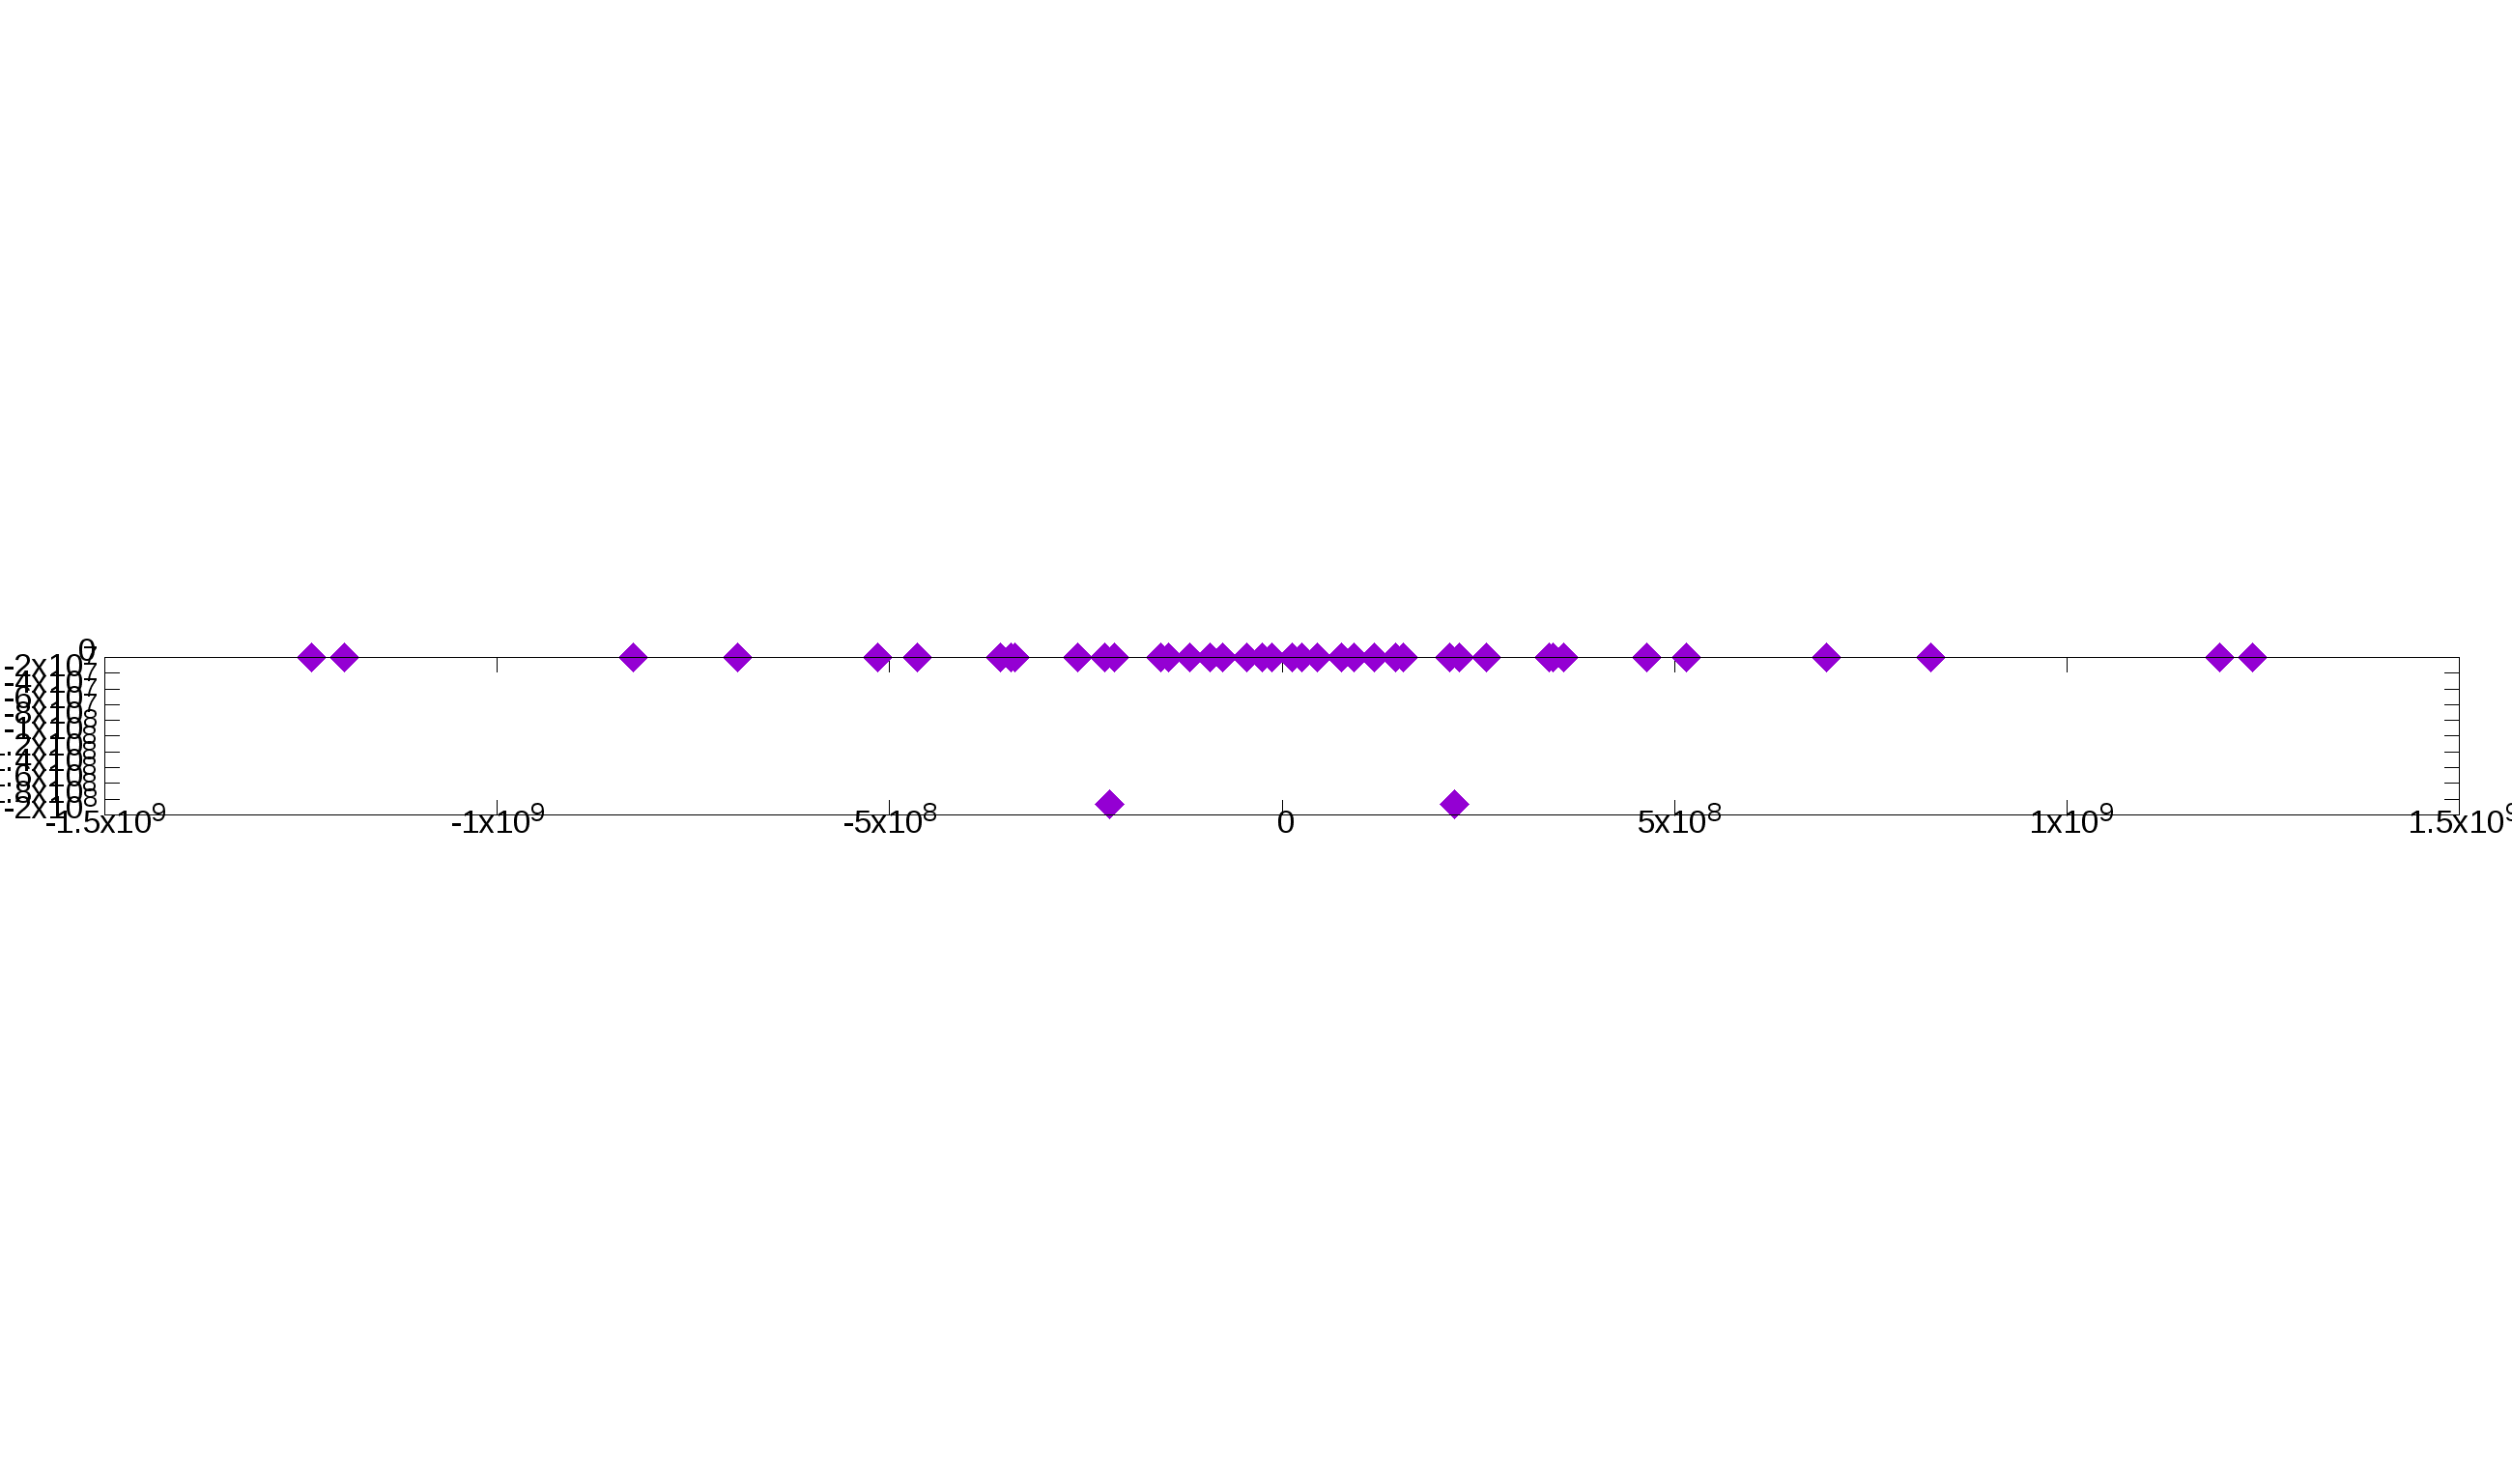
\includegraphics[width=1\linewidth]{./img/42_symm.png}}
\parbox{1\linewidth}{\caption{IPS of cardinality 42 and diameter 2473117504}
\label{42_symm.png}}
\end{figure}

\begin{figure}[h!]
center{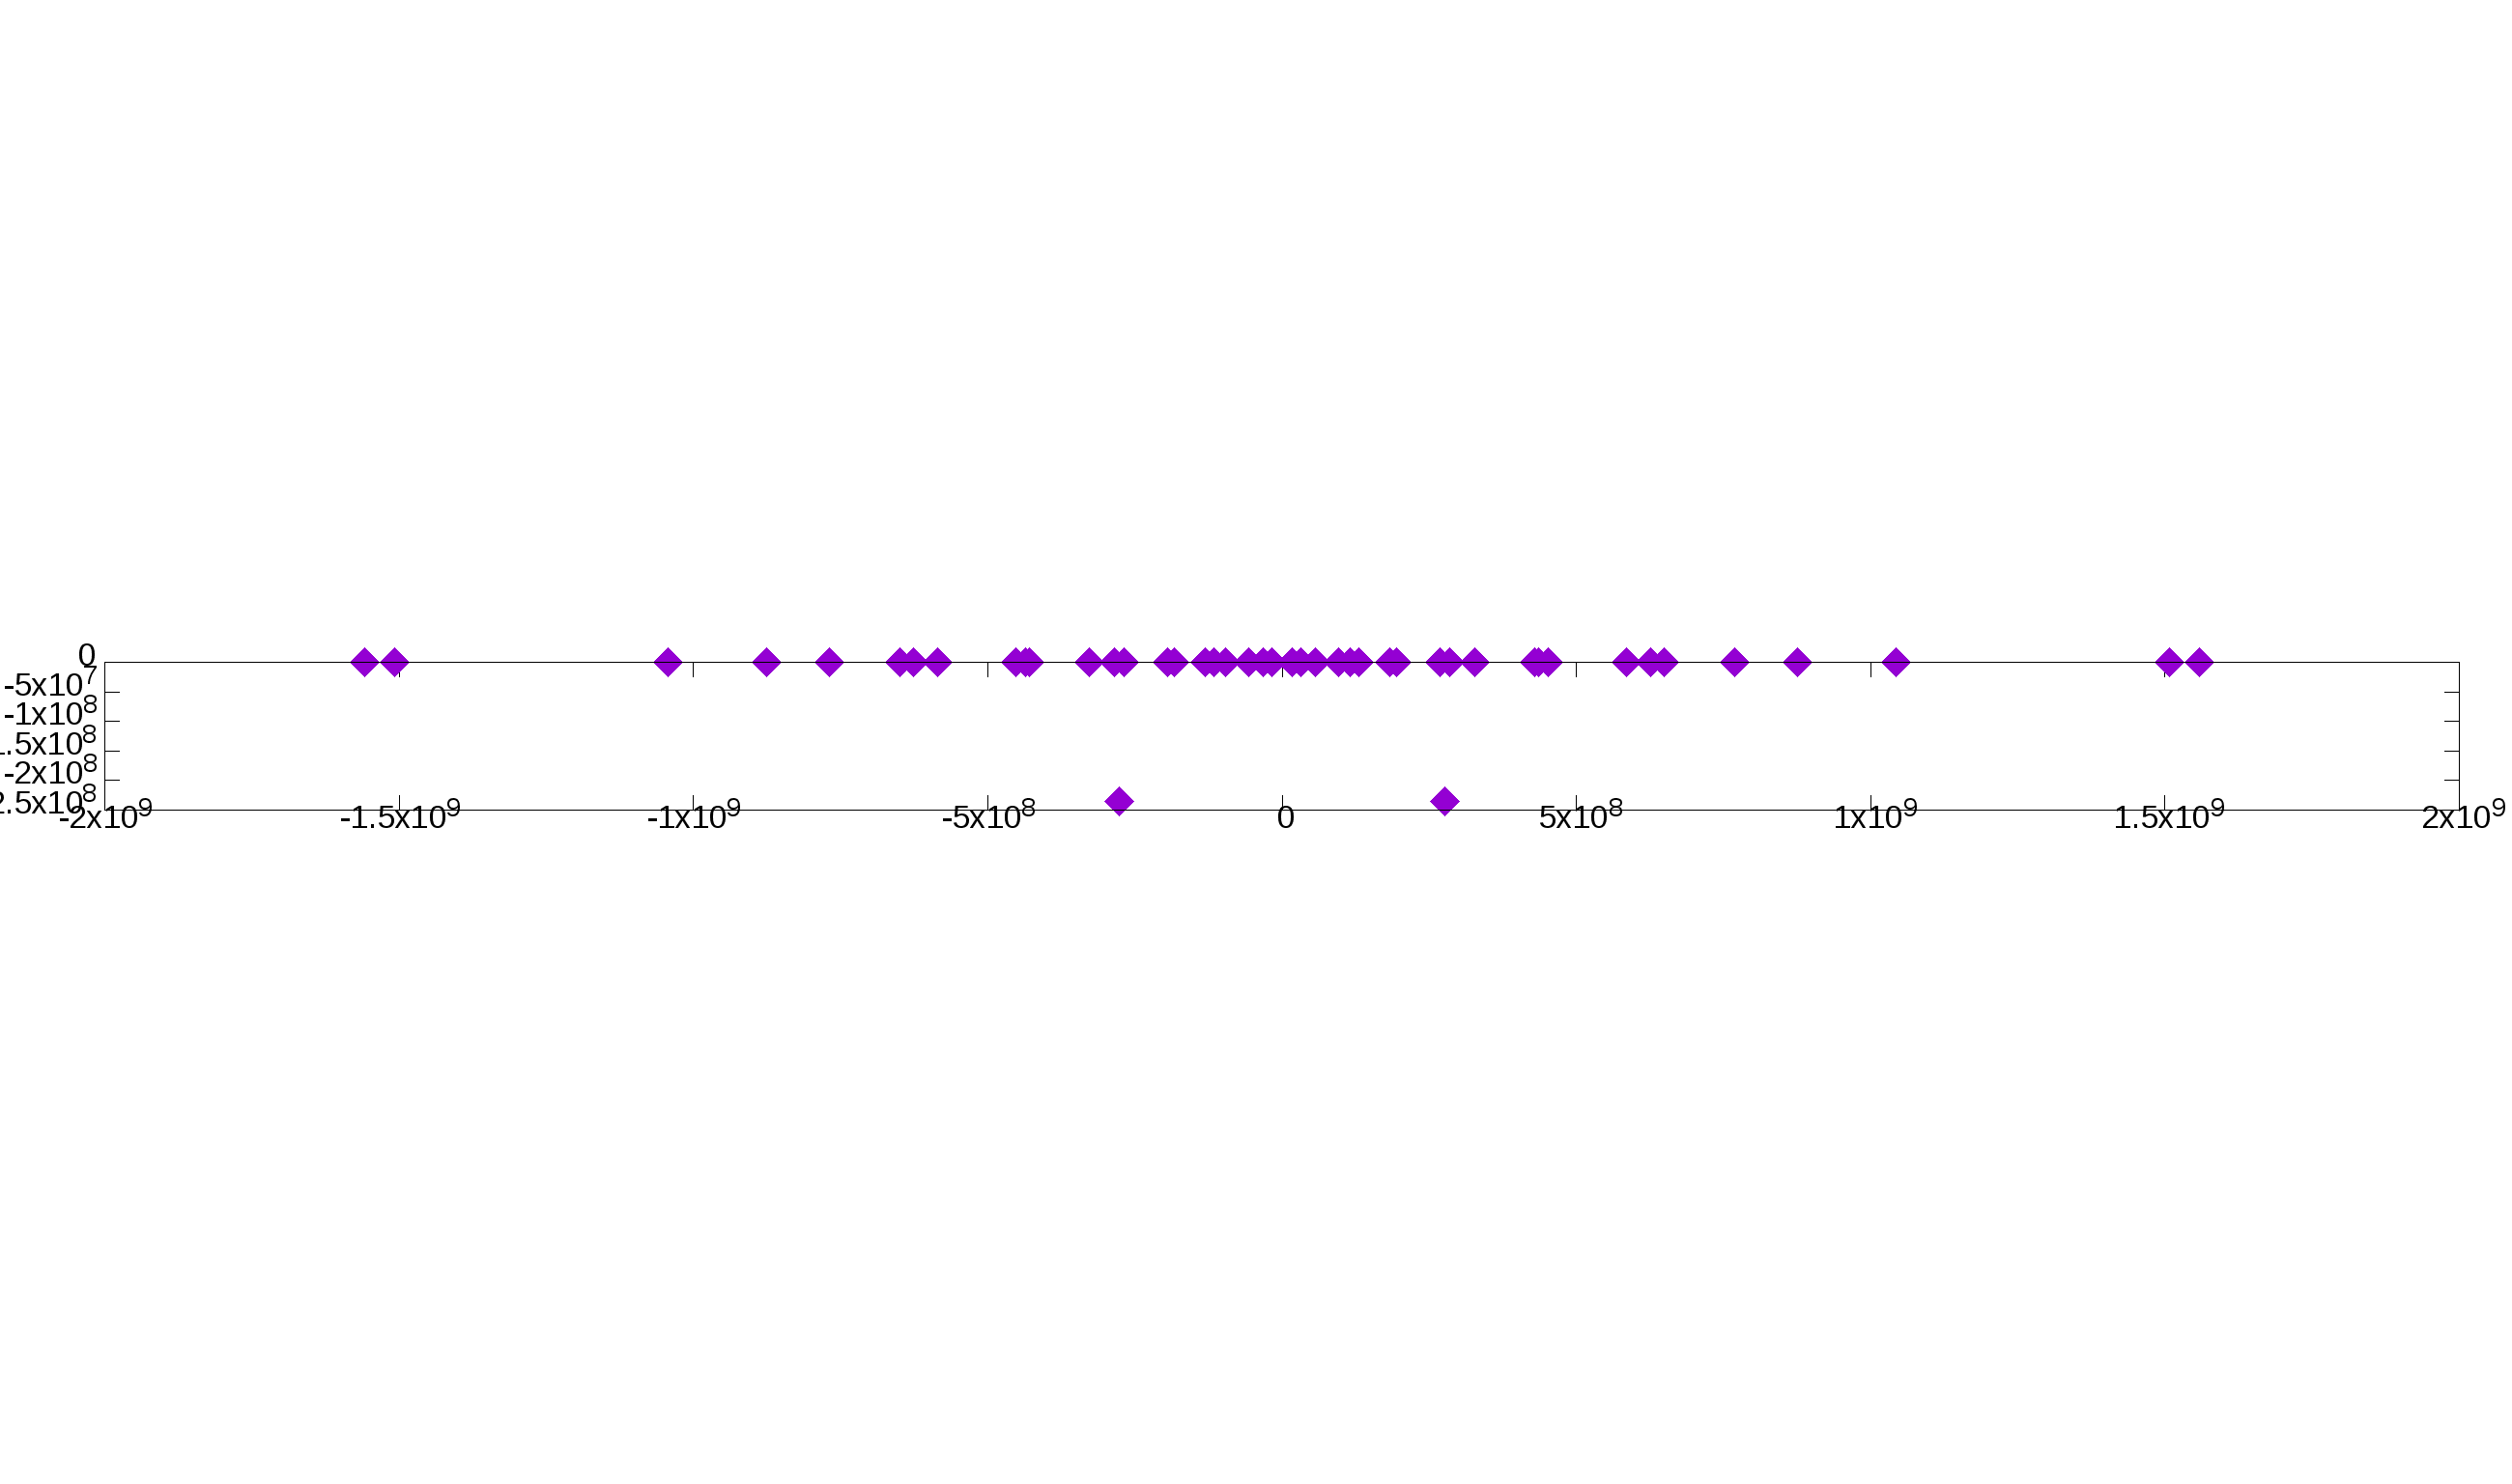
\includegraphics[width=1\linewidth]{./img/46_symm.png}}
\parbox{1\linewidth}{\caption{IPS of cardinality 46 and diameter 3118278592}
\label{46_symm.png}}
\end{figure}

\begin{figure}[h!]
center{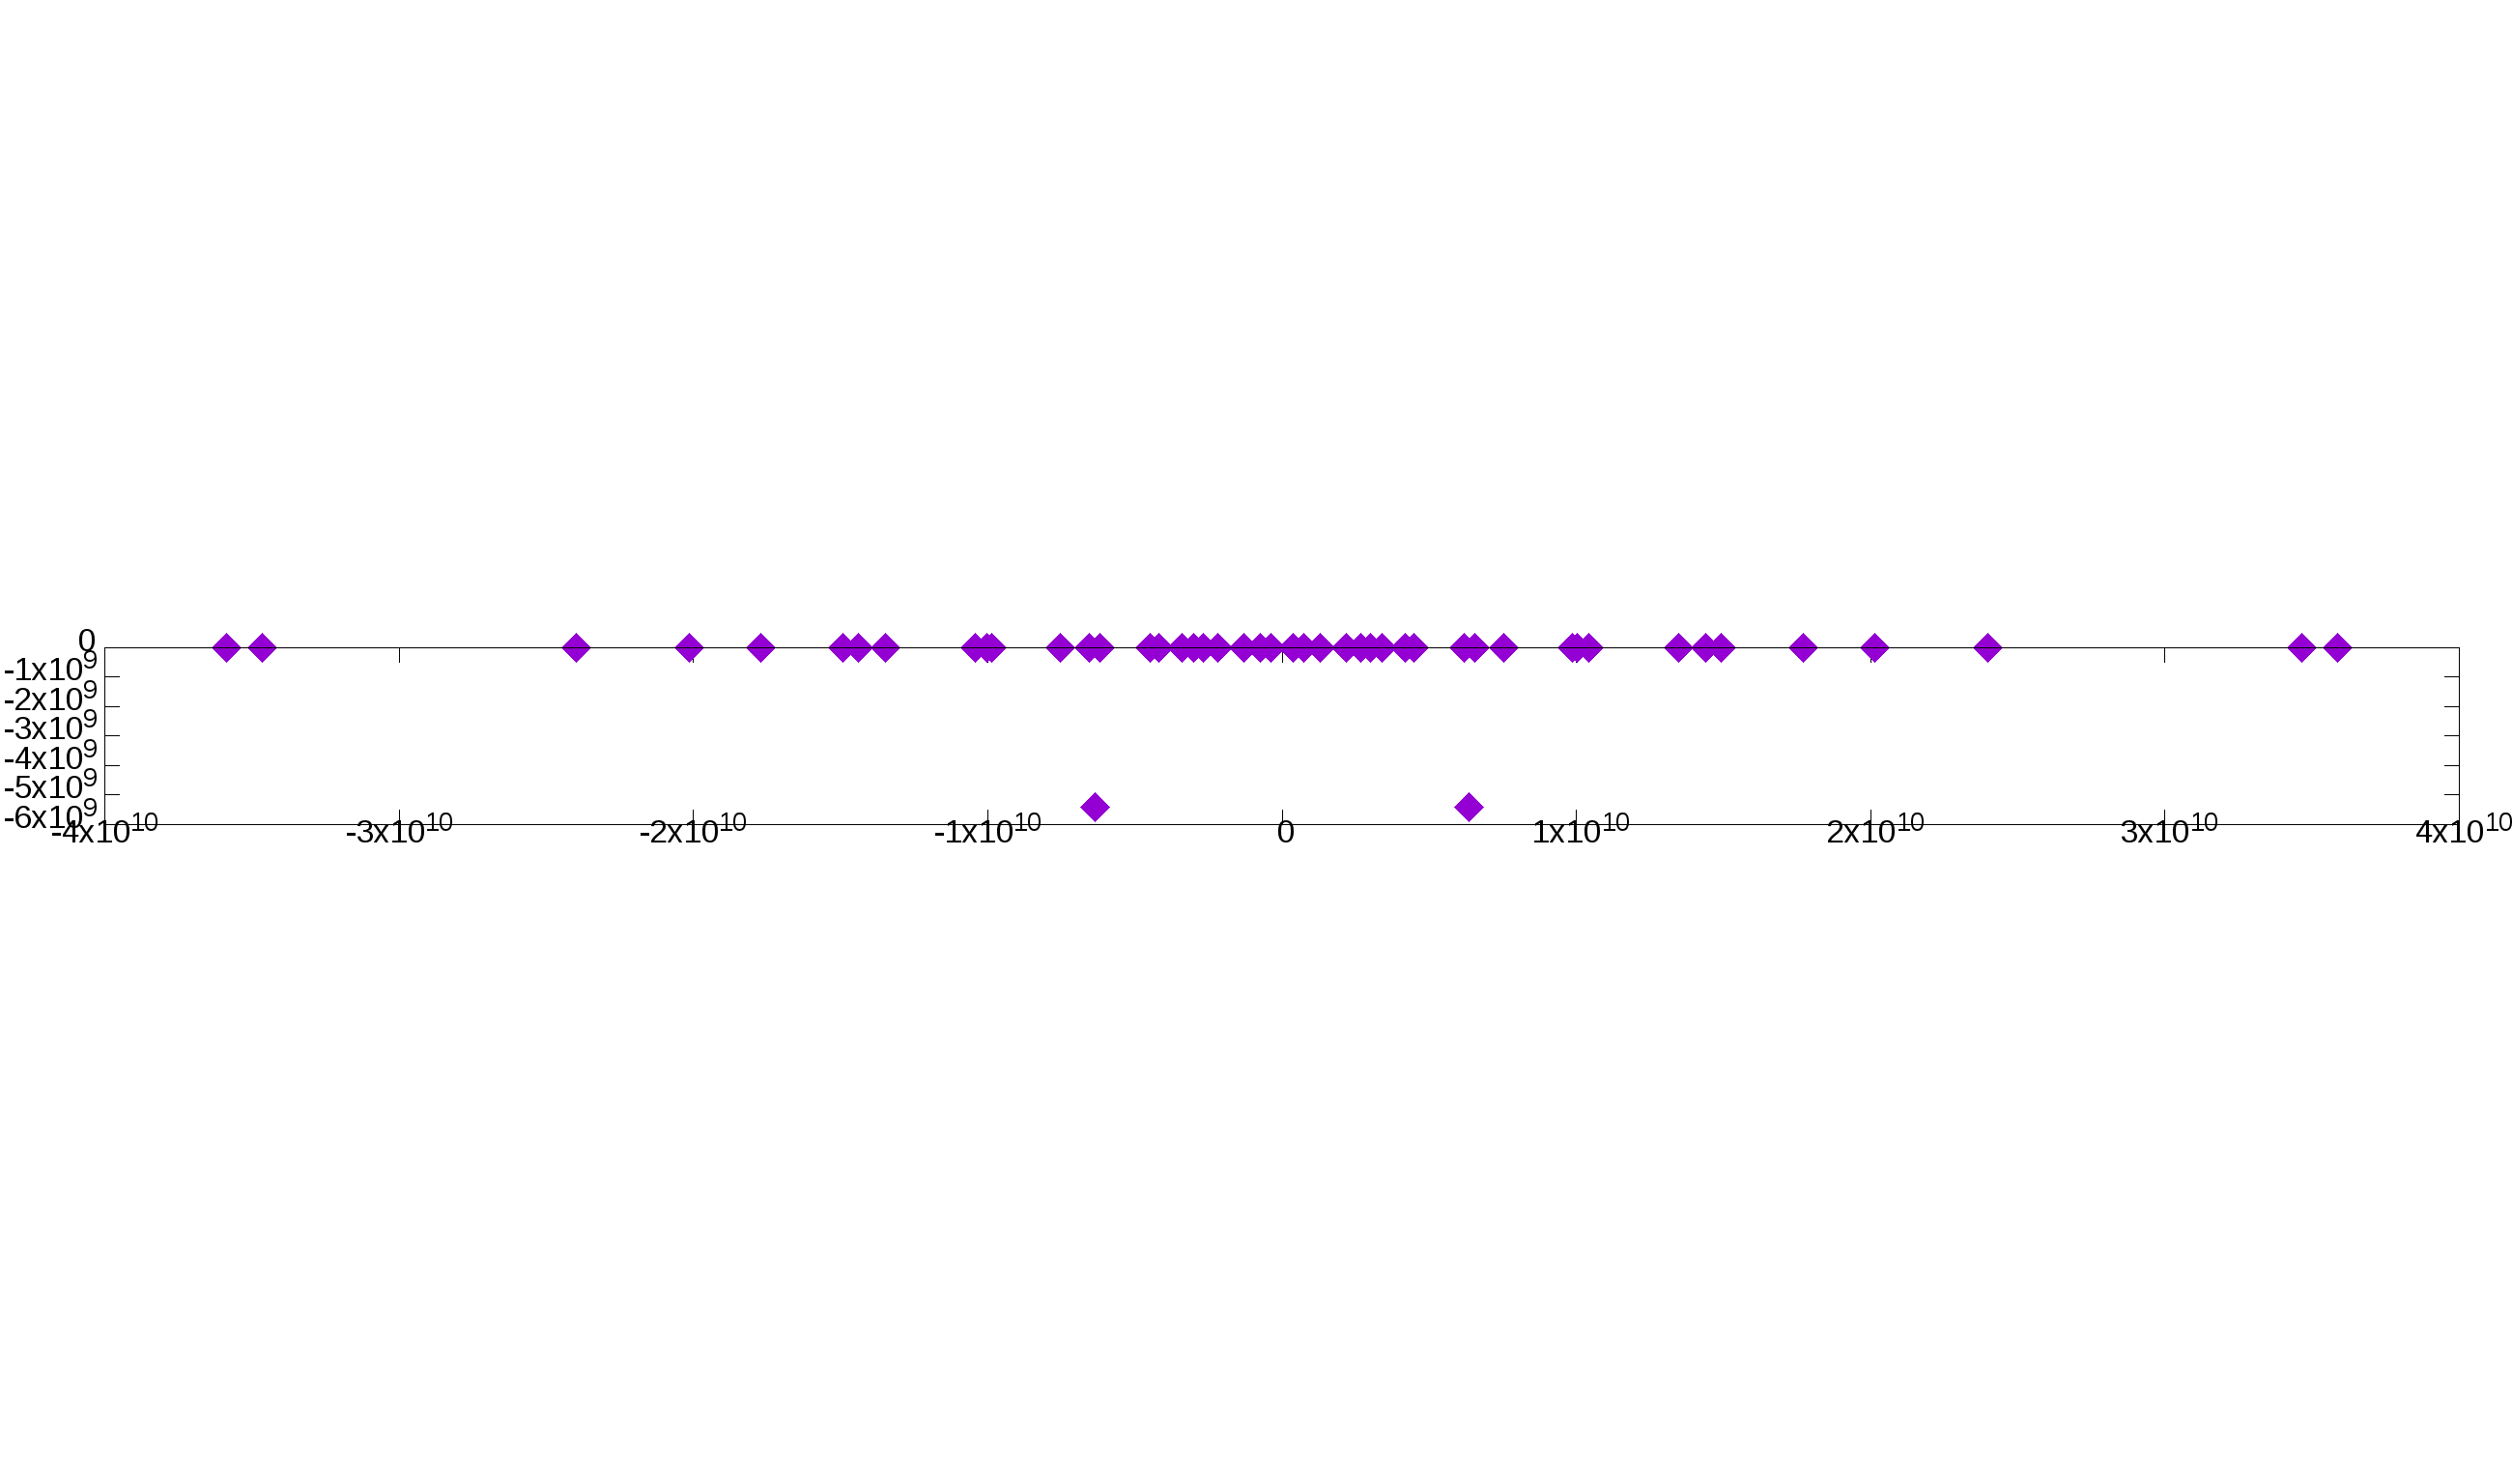
\includegraphics[width=1\linewidth]{./img/48_symm.png}}
\parbox{1\linewidth}{\caption{IPS of cardinality 48 and diameter 71720407616}
\label{48_symm.png}}
\end{figure}

\begin{itemize}
\setlength{\itemsep}{-1mm}


\item
$\mathcal{P}=\sqrt{154}/{1} * \{ (\pm 345596160; 0);
(\pm219513840 -15069600);
(\pm260201760; 0);
(\pm225792840; 0);
(\pm213234840; 0);
(\pm153961080; 0);
(\pm144668160; 0
(\pm25116000; 0);
(\pm694026840; 0);
(\pm514710560; 0);
(\pm359116940; 0);
(\pm13423904; 0);
(\pm75682880; 0);
(\pm464143680; 0);
(\pm827069880; 0);
(\pm92144325; 0);
(\pm1195180740; 0);
(\pm1236558752; 0);
(\pm44590560; 0);
(\pm339925740; 0);
(\pm117312468; 0)\}
$
(Figure~\ref{42_symm.png}),

where $n = 42$, $\operatorname{diam(\mathcal{P})} = 2473117504$. Using the ``blowing up''
construction, we obtain
\begin{equation}\label{result2}
d(m, 3m + 1) \leq 56
\end{equation}
The resulting estimate improves the estimate for $d(m, 3m)$, which is presented
in \cite{kemnitz1988punktmengen}. Figure~\ref{picture_12.pdf} shows an example
for $m = 3$.


\item
$\mathcal{P}=\sqrt{154}/{1} * \{ (\pm435751680; 0);
(\pm276778320; -19000800);
(\pm328080480; 0);
(\pm284695320; 0);
(\pm268861320; 0);
(\pm194124840; 0);
(\pm182407680; 0);
(\pm31668000; 0);
(\pm1559139296; 0);
(\pm1506967020; 0);
(\pm1042827240; 0);
(\pm875077320; 0);
(\pm648982880; 0);
(\pm585224640; 0);
(\pm452799620; 0);
(\pm95426240; 0);
(\pm16925792; 0);
(\pm116181975; 0);
(\pm428602020; 0);
(\pm56222880; 0);
(\pm769560480; 0);
(\pm626458560; 0);
(\pm130761918; 0)\}
$
(Figure~\ref{46_symm.png}),

where $n = 46$, $\operatorname{diam(\mathcal{P})} = 3118278592$. Using the ``blowing up''
construction, we obtain
\begin{equation}\label{result3}
d(m, 4m + 1) \leq 1260
\end{equation}
Figure~\ref{picture_1260_R3.pdf} shows an example for $m = 3$.

\item
$\mathcal{P}=\sqrt{154}/{1} * \{ (\pm10022288640; 0);
( \pm6365901360 ; -437018400); 
( \pm7545851040 ; 0); 
( \pm6547992360 ; 0); 
( \pm6183810360 ; 0); 
( \pm4464871320 ; 0); 
( \pm4195376640 ; 0); 
( \pm728364000 ; 0); 
( \pm35860203808 ; 0); 
( \pm34660241460 ; 0); 
( \pm23985026520 ; 0); 
( \pm20126778360 ; 0); 
( \pm14926606240 ; 0); 
( \pm13460166720 ; 0); 
( \pm10414391260 ; 0); 
( \pm2194803520 ; 0); 
( \pm389293216 ; 0); 
( \pm2672185425 ; 0); 
( \pm9857846460 ; 0); 
( \pm1293126240 ; 0); 
( \pm17699891040 ; 0); 
( \pm14408546880 ; 0); 
( \pm3007524114 ; 0); 
( \pm3402061572 ; 0)\}
$
(Figure~\ref{48_symm.png}),

\end{itemize}

\section{Final remarks}
All the given PIPSs were obtained through a combination of computer search an intuition of the authors;

There is still no general construction for a rails or scissors PIPS of given cardinality.
For rails PIPSs, we can conjecture that there exists a set of arbitrary cardinality with 2 points on one line
and all the rest on the other;
on the other hand, we still have not found any rails PIPSs with 4 and 5 points on the lines.


The source code can be obtained at https://gitlab.com/Nickkolok/ips-algo

\printbibliography
%\bibliography{literature}

\end{document}
